% begin module trig-example
\begin{frame}
\begin{example}
\begin{columns}[c]
\column{.5\textwidth}
\ \only<handout:0| -1>{%
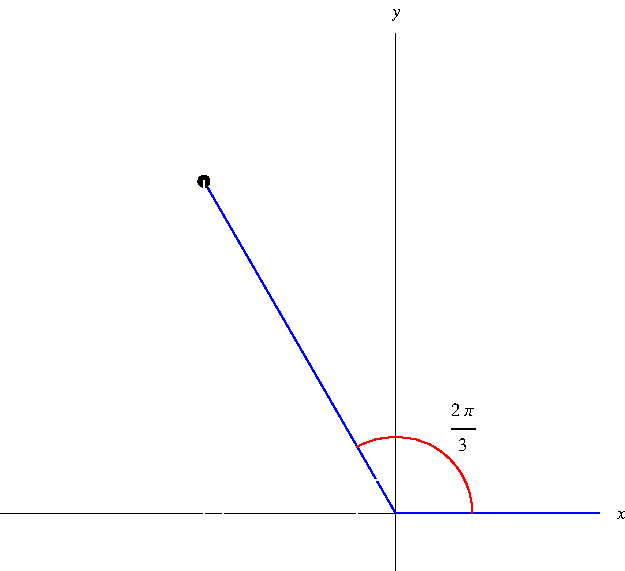
\includegraphics[width=5cm]{trigonometry/pictures/app-d-ex3a.pdf}%%
}%
\only<handout:0| 2>{%
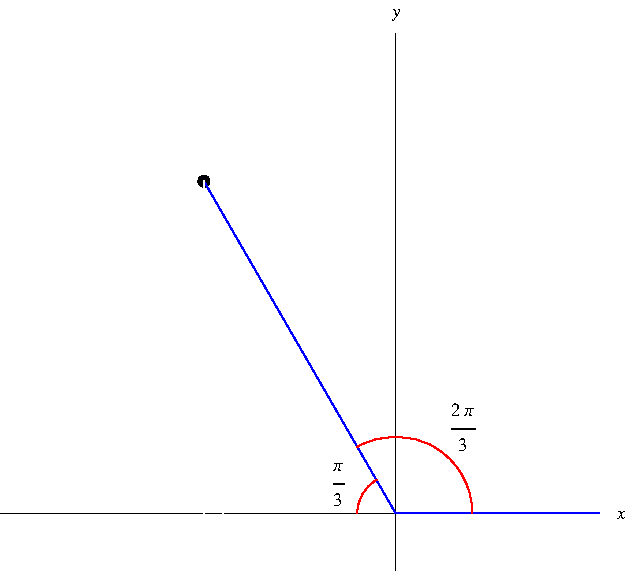
\includegraphics[width=5cm]{trigonometry/pictures/app-d-ex3b.pdf}%%
}%
\only<3->{%
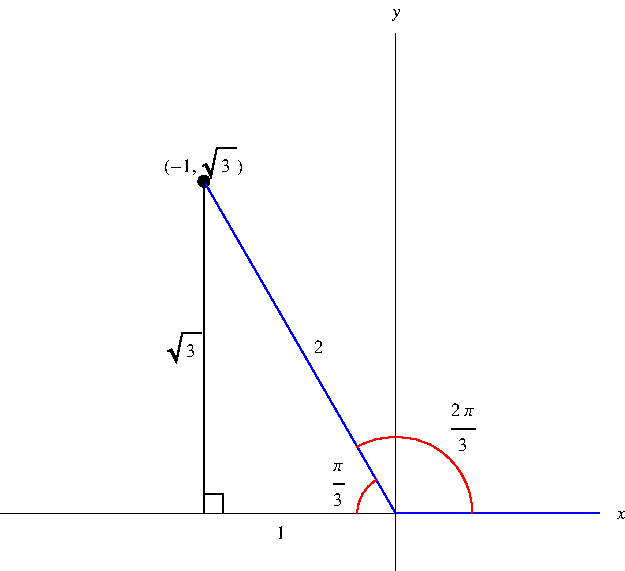
\includegraphics[width=5cm]{trigonometry/pictures/app-d-ex3c.pdf}%%
}%
\column{.5\textwidth}
Find the exact trigonometric ratios for $\theta = 2\pi /3$.
\end{columns}
\begin{align*}
\alert<handout:0| 4-5>{\sin \frac{2\pi}{3}} & \alert<handout:0| 4-5>{= \uncover<5->{\frac{\sqrt{3}}{2}}} &
\alert<handout:0| 6-7>{\cos \frac{2\pi}{3}} & \alert<handout:0| 6-7>{= \uncover<7->{-\frac{1}{2}}} &
\alert<handout:0| 8-9>{\tan \frac{2\pi}{3}} & \alert<handout:0| 8-9>{= \uncover<9->{-\sqrt{3}}} \\
\alert<handout:0| 10-11>{\csc \frac{2\pi}{3}} & \alert<handout:0| 10-11>{= \uncover<11->{\frac{2}{\sqrt{3}}}} &
\alert<handout:0| 12-13>{\sec \frac{2\pi}{3}} & \alert<handout:0| 12-13>{= \uncover<13->{-\frac{2}{1}}} &
\alert<handout:0| 14-15>{\cot \frac{2\pi}{3}} & \alert<handout:0| 14-15>{= \uncover<15->{-\frac{1}{\sqrt{3}}}}
\end{align*}
\end{example}
\end{frame}
% end module trig-example
